
%%%%%%%%% Section 2.4
\subsection{Comparison to Other Methods}\label{sec:othermethods}
We establish two comparisons: first to Bayesian inversion \cite{Walpole, Berger, Complete, Smith}, the second to a measure-theoretic approach studied in \cite{BET+14, BE13}.


\subsubsection{Statistical Bayesian Approach}

%If the quantity of interest is a single measurement, then the likelihoods and observed densities are identical.
%However, the quantity of interest may not necessarily just be the uncertainty in the measurement data, as we will see in later discussions.
%For completeness, we define the alternative solution to the SIP below and compare the two frameworks under a simple linear map.

The Bayesian formulation gives a posterior density as:

\begin{equation}\label{eq:sb_post}
    \pp\lam := \initial\lam \frac{L_\dspace (d | \param)}{ C },
\end{equation}

where we use $\pp$ to distinguish the \emph{posterior} from the updated density $\updated$ in \eqref{eq:update}.

Here, we borrow the notation $\initial$ to represent the Bayesian $\pp_\text{prior}$, since in our comparative examples we use the two interchangeably.
We choose them to represent the set of feasible parameters, and rely on Monte-Carlo sampling for both approaches\footnote{Priors in Bayesian inference are sometimes chosen for reasons related to Markov-Chain Monte-Carlo algorithms in order to ensure their balancing of investigation and exploration, or convergence [TK - cite someone]}.


$L_\dspace$ is the likelihood function as a function of the output and the denominator $C$ is a \emph{normalizing constant}, chosen so that the updated density integrates to one, namely
\[
C = \int_\pspace \initial\lam L_\dspace(d | \param) \, d\param.
\]

Note that the likelihood function is not necessarily a density.
In fact, $L_\dspace$ need not even be in $L^1(\pspace)$ since it is actually only the product $\initial(\param) L_\dspace (d | \param)$ that is required to be in $L^1(\pspace)$ to form a posterior.
In other words, $L_\dspace (d | \param)$ and $\observed(\qlam)$ can model completely different things with respect to uncertainty in the data. 
An interpretation of $L_\dspace (d | \param)$ is the relative likelihood that a single parameter $\param\in\pspace$ explains the observed data, whereas $\observed(\qlam)$ describes the relative likelihood of a predicted datum associated with $\param\in\pspace$.

It is important to note that the Bayesian framework poses a different question for which a different answer is sought, which is based on the presence of $L_\dspace(d | \param)$ in place of $\observed(\qlam)$.
Specifically, the problem analyzed by the Bayesian approach is to determine a single ``true'' parameter that explains all of the observed data \cite{Smith, Concrete, Complete}.
In this framework, there is a different notion of consistency, referring to certain asymptotic properties of $\updated$ in the limit of infinite data \cite{Barron, Silverman}.
The philosophical underpinnings of Bayesian inference\---the underlying question being asked\---is akin to the following:

\begin{center}
  \emph{How does one incorporate collected data to shift prior beliefs about parameter values?}
\end{center}

This is in contrast to the Data-Consistent framework, where we seek a pull-back measure: a description of the uncertainty set that explains the variation in the observations under a given description of error.
This approach expresses a desire to reconstruct a distribution (or probability measure), asking:

\begin{center}
  \emph{How does one update prior beliefs in such a way that modifies predictions to match the description of uncertainty in observed data?}
\end{center}

We note that there are problems that one can formulate where the observed density corresponds directly to a normalized likelihood function familiar to Bayesian statisticians, as we demonstrate below.

One difference that is immediately obvious between the two solutions is the use of normalizing constant $C$ in $\pp$ not present in $\updated$, as discussed in Corollary~\ref{cor:int} above.
To illustrate the two approaches, we explore the impact of this difference in the example below, taken from \cite{BJW18}.

\begin{ex}
Consider
\begin{equation}
u(\param) = \param^p
\end{equation}
for $p$ chosen as either 1 or 5.
For both approaches, the prior or initial density is given by $\initial \sim U[-1,1]$.
In the Data-Consistent Inversion framework, $\observed \sim \mathcal{N}(0.25,0.1^2)$.
In the statistical Bayesian framework, we take $d=0.25$ and assume an additive error noise model with distribution $\mathcal{N}(0,0.1^2)$ so that the likelihood, $L_\dspace(d | \param)$, matches the observed density as a function of $\param$.

When $p=1$, we have $\predicted = \frac{1}{2} = C$.
Since $\observed\q = L_\dspace(d|\param)$ and $\predicted$ agrees with the normalizing constant $C$, the posterior and update agree on $\pspace$ (we show the push-forwards in the right plot of Figure~\ref{fig:comparison}).
When $p=5$, the non-linearity of the model causes the push-forward of $\initial$ to be non-constant, so the two approaches now yield differing solutions, as seen in the left plot of Figure~\ref{fig:comparison}).
The push-forward of the posterior associated with the statistical Bayesian framework is influenced by the push-forward of the prior in a way that the push-forward of the updated density avoids.

\begin{figure}
\begin{minipage}{.45\textwidth}
		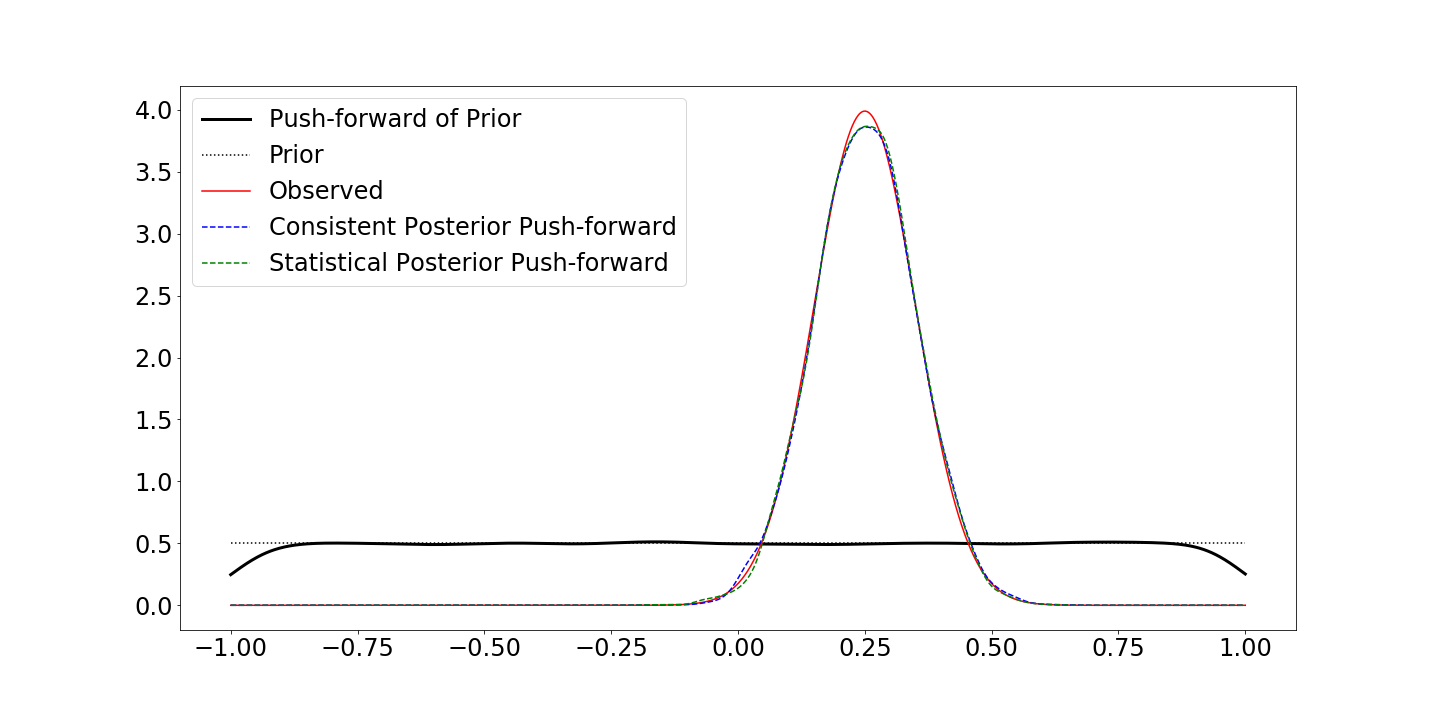
\includegraphics[width=\linewidth]{./images/comparison1}
\end{minipage}
\begin{minipage}{.45\textwidth}
		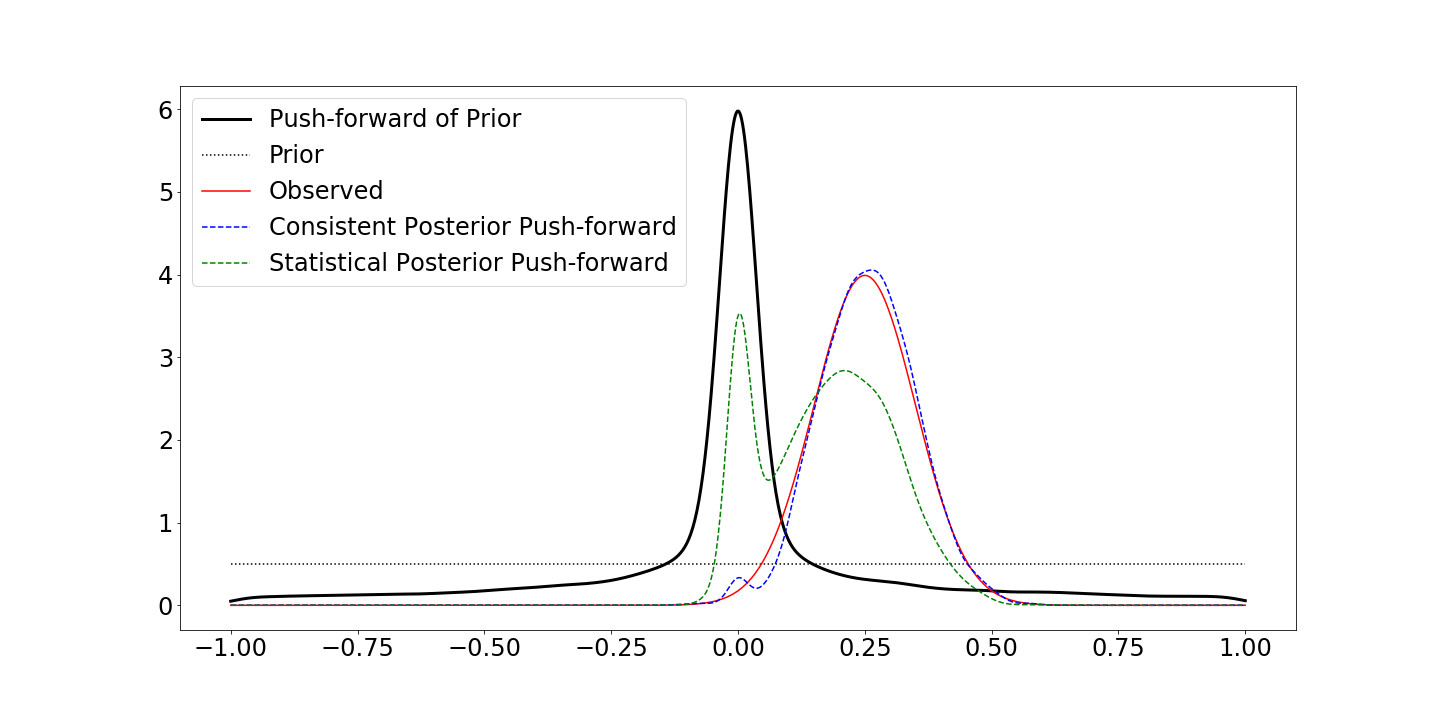
\includegraphics[width=\linewidth]{./images/comparison5}
\end{minipage}
\caption{
In each plot, the black dotted line represents the prior (initial), while the solid line represents the push-forward.
The push-forwards of the posterior (updated) densities are shown as a green (blue) dotted line.
The likelihood (observed density) is shown as a solid red line.
(Left): $p = 1$, the push-forwards of the solutions are identical because a linear map results in a constant push-forward of a uniform prior.
(Right): $p = 5$, the non-linearity of the map causes the solutions to be different and thus the push-forwards to also be different.
}
\label{fig:comparison}
\end{figure}

% [TK - removed paragraph] We can see in Figure~\ref{fig:comparison} that the two approaches pose different questions and thus yield different results.
% The Data-Consistent Inversion framework seeks to recreate the observed density, which it does for both $p=1$ and $p=5$, but the Bayesian approach is a combination of both the observed and the push-forward of the prior.

For the sake of fairness, it is worth noting that Bayesians do not push-forward their posterior density, so in some sense this comparison is not entirely fair.
It is not the goal of Bayesian inference to recreate the likelihood function in this way.
Rather, the point of maximum likelihood would be propagated and perturbed with the assumed noise model.
This is because Bayesian inverse problems are fundamentally posed as parameter-identification (an optimization to be performed), not distribution estimation.
In the event that a Bayesian would want to estimate a distribution, they would do so by creating a parametric representation thereof.
For example, one could assume that a posterior on $\pspace$ can be expressed as a Gaussian distribution, and solve for the most likely mean and standard deviation that characterizes it [TK - cite more] \cite{Smith}.
Nonparametric densities can be approximated by mixture models.
For example, one can assume that the posterior can be given by a linear combination of four Gaussian distributions, and solve for eight parameter values (four standard deviations and means).
However, the operative word here is \emph{assume}; in order to capture a density using a Bayesian framework, one needs to impose some sort of explicit structure on the posterior.
No such compromise is required in the Data-Consistent Inversion framework.
Distributions (or measures) can be solved for directly, regardless of any nonlinear/non-parameteric structure by leveraging the measure-theoretic approach described in \cite{BE13} or \cite{BJW18}.

\end{ex}
